


\chapter{Mathematical Flexibility\label{ch:math}}
%-----------------------------------------------------------------------------

Introducing formal methods into a software engineering project causes a sharp increase in the up-front effort required to develop the software.  Appropriate and sound mathematical theories must be developed, components must be formally specified by a software engineer trained in formal techniques, and verification conditions must be dispatched by a mathematician in a formal environment that eliminates the possibility of human error, possibly with the assistance of an automated proving tool.

While we argue that this cost is justified in critical or long-running deployments by a corresponding reduction in effort during the maintenance phase of the software lifecycle, it is undeniable that this remains a barrier for entry to many projects that could otherwise benefit from formal methods of quality assurance.  The hypothesis is that a number of steps could be taken to reduce the real or percieved additional effort, as well as increase the corresponding long-term benefits.

%-----------------------------------------------------------------------------
\section{General Design Goals\label{mathDesignGoals}}
%-----------------------------------------------------------------------------

After considering the problem, we arrived at three overarching strategies to address verificaton complexity, then considered a number of features that would support these objectives.  This section covers the overarching strategies, while the next lists specific features and explains how they support these strategies. 

	%---------------------------------------------------------------------
	\subsection{Usable Theories\label{usableTheories}}
	%---------------------------------------------------------------------

Certainly the most straightforward way of addressing the complexity issue is simply to reduce the effort associated with formal verification.  The central mathematical challenges in developing verified software may generally be understood to arise from two sources: \emph{producing} mathematical content, which includes writing sound and sufficiently complete theories, along with utilizing them in specifications; and \emph{employing} mathematical content, which mostly manifests as the dispatching of verification conditions, either by hand or via an automated prover.

The complexity of developing mathematical theories and specifications may be addressed by making it as easy as possible to work with the mathematical subsystem of the verification tool.  \emph{Familiarity} is the most obvious kind of ease.  It encompasses both syntax and environment.  Because the target users of the RESOLVE mathematical subsystem are mathematicians, we strive to make the RESOLVE theory language look and behave as much like traditional mathematics as possible.  Another kind of ease is \emph{tool support}, wherein the compiler assists the user in spotting and correcting errors.

The complexity of the verification problem may be addressed by making VCs easier to dispatch.  While the subject of increasing the power of the automated prover to encompass more VCs is the topic of Chapter \ref{ch:prover} of this dissertation, we can affect this effort in the theory development domain by creating theories that result in \emph{more straightforward} VCs.  This is the process we term \emph{specification engineering}, which encompasses techniques such as choosing appropriate abstractions, limiting quantifier use, and appropriate theory modularity, all of which necessitate the significant amounts of mathematical flexibility introduced in this chapter.

	%---------------------------------------------------------------------
	\subsection{Modular Theories\label{modularTheories}}
	%---------------------------------------------------------------------

Borrowing from the software development world, we note that when complexity is unavoidable, it can be mitigated by strong modularity in the form of clear demarcations between atomic conceptual units.   Such units serve both to organize the thoughts of the human user and to provide a finer granularity with which to import such concepts, decreasing the clutter in namespaces and ensuring that only the resources that are truly needed are brought into context.  In the presence of an automated prover, we hypothesize that such a strategy assists the ease with which VCs can be dispatched by ensuring that the prover only considers those theorems relevant to the current domain.

Note that it's not our desire to place on the user the burden of deciding which mathematical results might be relevant, but rather to ensure that appropriate theorems are bundled with the mathematical objects upon which they operate.  A user might work with binary relations a great deal, but only when she wishes to use the \texttt{Is\_Total\_Preordering} predicate would she import \texttt{Preordering\_Theory}.  By importing what is necessary to gain access to such a predicate, she also gains a body of mathematical results for reasoning about such relations.

	%---------------------------------------------------------------------
	\subsection{Reusable Theories\label{reusableTheories}}
	%---------------------------------------------------------------------

A theory or component that enjoys continuous reuse amortizes over time the up-front effort required to create and verify it.  We therefore have saught to create and add those features that would permit the development of reusable theories, types, theorems, and components.  Such a strategy both decreases the effort required to create new theories and increases the liklihood that an existing theory is already available that can meet the user's needs.  In seeking out such features, we draw from the body of existing programming languages techniques, including encapsulation, polymorphism, and inheritance, and seek to adapt them for theories and specifications.


%-----------------------------------------------------------------------------
\section{Preliminaries\label{preliminaries}}
%-----------------------------------------------------------------------------

Before discussing the concrete features that address these general goals, it is useful for the sake of clarity and brevity to explain a few important concepts and notational conveniences that we will use for the remainder of this chapter.
	%-----------------------------------------------------------------------------
	\subsection{Objects \emph{vs.} Expressions\label{objectsVsExpressions}}
	%-----------------------------------------------------------------------------

We will occasionally need to distinguish between a \emph{mathematical value and its corresponding type} and a \emph{RESOLVE expression and its corresponding type}.  The former is a mathematical object representable in the universe of RESOLVE.  The latter is a meta-concept pertaining to syntax.  When we wish to indicate a mathematical value, we will use the standard mathematical syntax.  E.g., $\forall i : \mathbb{Z}, ...$ quantifies over all mathematical integers.  When we wish to indicate a RESOLVE expression of some type, we will use the meta-type \textbf{Exp}, subscripted with the type of the expression.  E.g., $\forall i : \textbf{Exp}_\mathbb{Z}, ...$ quantifies over all RESOLVE expressions that, when evaluated, would yield a mathematical integer.  We will also use the meta-function \emph{Eval}, which takes an \textbf{Exp} and returns the results of evaluating the expression.
	%-----------------------------------------------------------------------------
	\subsection{Operating on Expressions\label{operatingOnExpressions}}
	%-----------------------------------------------------------------------------

\begin{sloppypar}
When normal mathematical functions (e.g., $\cup$, $\times$, etc.) are shown operating on \textbf{Exp}s, this is a shorthand for constructing a new RESOLVE expression resembling the given expression, with any \textbf{Exp}-valued variables macro-expanded into their full expression values.  For example, the assertion $\forall~R,~T~:~\textbf{Exp}_{\mathcal{P}(\mathbb{Z})},~\text{Eval}(R~\cup~T)~\supseteq~\text{Eval}(R)$ does not contain an attempt to somehow ``union'' two expressions ($\cup$ operates on types, not expressions), but rather constructs a new union expression with $R$ and $T$ as sub-expressions.
\end{sloppypar}
	%-----------------------------------------------------------------------------
	\subsection{Type Equality\label{typeEquality}}	
	%-----------------------------------------------------------------------------

Equality of types can be a complex topic.  In this text, when we say, for some types $T$ and $R$, that $T~=~R$ (or use the word ``equals'') we mean that $T$ and $R$ are \emph{alpha-equivalent}.  Two types are alpha-equivalent if they are identical except for the names of any quantified variables, which may be different so long as they do not change the internal relationships among the variables (i.e., the names can not be changed to make two previously differently-named variables the same.)


%-----------------------------------------------------------------------------
\section{Concrete Features\label{mathFeatures}}
%-----------------------------------------------------------------------------

	%---------------------------------------------------------------------
	\subsection{Higher-order Logic\label{higherOrderLogic}}
	%---------------------------------------------------------------------

The availability of first-class functions in theories and specifications both increases mathematical \emph{familiarity} (supporting usability) and encourages patterns of reuse.  Specifications of non-trivial reusable software components and patterns supported in programming languages are difficult or impossible to specify or verify using the first-order logic dictated by most practical verification systems and automated provers.  For example, the Strategy patten, functional constructs, and program templates all become impossible to specify.

Higher-order logic has long been the norm in the functional language and proof assistant community where a small core logic and extensibility have been a focus.  A fascinating history is presented in \cite{gordon2000lcf} tracing such systems from Robin Milner's original Logic of Computable Functions system\cite{milner1972implementation}, which is based on first-order logic, through the original motivations in hardware verification for expanding and updating that system into what would become HOL\cite{gordon1993introduction}, a higher-order logic proof assistant.  HOL would become the predecessor to Isabelle\cite{nipkowIsabelle}.

Despite this near-ubiquity of higher-order logic in the realm of pure systems, it is not often found in practical ones.  This is in large part due to the inability of SMT-solvers, which form the backbone of most practical systems due to their efficiency, to be applied soundly to proving higher-order assertions.  This limitation and a technique for mitigating it are discussed in \cite{fontaine2006expressiveness}.

As discussed in Chapter \ref{ch:prover}, our minimalist prover leaves functions and definitions \emph{uninterpretted}.  A function or definition is uninterpretted when we do not expand it to consider its definition---i.e., the mathematical subsystem looks at a function or definition variable as a black box, treating it no differently from an ordinary variable.  As a result, quantifying over functions introduces no additional complexity.  The tradeoffs inherent in such a design decision are discussed more completely in \cite{tagoreExpand}.

In addition to the familiarity gained by permitting mathematicians to treat functions as first-class citizens, their presence introduces a number of dimensions of usability and reuse:

		%------------------------------------------------------------
		\subsubsection{Higher-order Theorems\label{higherOrderTheorems}}
		%------------------------------------------------------------

Consider, for example the $foldr$ function ubiquitous in functional languages.  $foldr$ takes as its parameters a starting value of type $\gamma$, a function of type $(\gamma*\delta)\rightarrow\gamma$, and a list of elements of type $\delta$.  Begining with the starting value and the first element of the list, the function is applied to yield a new value of type $\gamma$ before repeating the procedure with the resultant value and the next element of the list.  The result of the final function application is returned.  A summing function for lists of integers could thus be defined as:

$sum(zs) = foldr(0, +, zs)$

The broad applicability of such a function for specification should be obvious.  However, even simple theorems describing the mathematical properties of this function run afoul of the first-order restriction that functions may not be quantified over.  For example, Theorem \ref{thm:foldremptylist} states that $foldr$ applied with an initial value to an empty list simply returns the initial value:

\begin{thm}
$\forall f : (\gamma*\delta)\rightarrow\gamma, \forall ds : List(\delta), (|ds| = 0) \Rightarrow (foldr(i : \gamma, f, ds) = i)$
\label{thm:foldremptylist}
\end{thm}

Higher-order specification languages such as RESOLVE permit such a theorem, enabling the development of a \emph{theory} of $foldr$, that in turn permits the automated prover to reason about expressions using such an expression at a high level of abstraction.

		%------------------------------------------------------------
		\subsubsection{Generic Theories of Functions\label{genericTheoriesFunctions}}
		%------------------------------------------------------------

Quantifying over functions also provides a straightforward mechanism for developing bodies of theorems that may be quickly applied to a new function.  This permits a number of useful properties to be proved once in the general case, and then be reused over multiple different instantiations.  Consider this snippet from \texttt{Preordering\_Theory}:

\newcommand{\reflexiveTheorem}{Preorder\_Reflexive}
\newcommand{\totalTheorem}{Total\_Preorder\_Is\_Total}

\begin{lstlisting}
Precis Preordering_Theory;

	Definition Is_Total_Preordering(f : (v1 : (D : MType) * v2 : D) -> B) : B;

	Theorem [*\totalTheorem*]:
		For all D : MType,
		For all f : D * D -> B,
		For all x, y : D,
			Is_Total_Preordering(f) implies
				f(x, y) or f(y, x);

	Theorem [*\reflexiveTheorem*]:
		For all D : MType,
		For all f : D * D -> B,
		For all x : D,
			Is_Total_Preordering(f) implies
				f(x, x);

	Theorem Preorder_Transitive:
		For all D : MType, 
		For all f : D * D -> B,
		For all x, y, z : D,
			Is_Total_Preordering(f) implies
				Is_Transitive(f);

end;
\end{lstlisting}

Now imagine we are defining a new operator, \texttt{Compare\_Zero\_Count}, which takes two \texttt{Str}s of $Z$ and compares the number of occurances of zero:

\begin{lstlisting}
Definition Compare_Zero_Count(S1 : Str(Z), S2 : Str(Z)) : B;
\end{lstlisting}

Clearly, such a function represents a total preording, and those are properties we may wish to rely on.  Rather than state the properties of a total-preordering again, specifically for this function, we may instead simply add:

\begin{lstlisting}
Theorem Compare_Zero_Count_Is_Total_Preordering:
	Is_Total_Preordering(Compare_Zero_Count);
\end{lstlisting} 

This theorem must be supported with a proof, of course, which requires that we establish that the function in question have the properties of transitivity and totality.  Following this, the full body of theorems available about total preorderings applies to \texttt{Compare\_Zero\_Count}.

It may at first seem that this is not much of a help---in order to use some of the theorems, we must first establish them, saving us no work.  However, note that the \texttt{\reflexiveTheorem} theorem is not a defining property of a total preordering, but rather follows from \texttt{\totalTheorem}.  Such theorems are now available for free with \texttt{Compare\_Zero\_Count}, because we are able to establish, once, in this module, that any function meeting the two properties of total preorder also meet these other theorems.

Note also that this arrangement decouples the decision of flagging a symbol with a particular property, and thus of including the entire body of results about that property, from the time of that symbol's definition.  This provides the option of allowing a third module to establish this relationship only when the property is semantically relevant, strengthening modularity.

		%------------------------------------------------------------
		\subsubsection{Extensible Specification\label{extensibleSpecification}}
		%------------------------------------------------------------

Inheritence is a powerful tool, but the cause of much problematic reasoning\cite{vlissides1995design}.  While RESOLVE does not support direct inheritence, a specification may provide points for extension by permitting function parameters that modify its behavior.  This, in turn, can permit a client to simplify their own reasoning while still using an off-the-shelf component.

As an example, consider the \texttt{Predicate\_Stack}, presented in Listing~\ref{lst:predStack}, which ensures a predicate holds on each of its elements.

\begin{lstlisting}[float=h,language=resolve,caption={A partial specification for \texttt{Predicate\_Stack}\label{lst:predStack}}]
Concept Predicate_Stack(Type Entry, Definition Predicate : Entry -> B);

	...

	Operation Push(alters E : Entry, updates S : Predicate_Stack);
		requires Predicate(E);
		ensures S = #S o <#E>;

	Operation Pop(replaces E : Entry, updates S : Predicate_Stack);
		requires |S| > 0;
		ensures #S = S o <E> and Predicate(E);

end;
\end{lstlisting}

Just as a type-parameterized stack component prevents the user from needing to reassure the type system of the types of elements as they are removed from the stack, a predicate-parameterized stack component prevents the user from engaging in complex gymnastics to assure the verification system of properties that hold on its elements each time they are removed---those properties may simply be assumed. 

		%------------------------------------------------------------
		\subsubsection{Strategy Pattern\label{strategyPattern}}
		%------------------------------------------------------------

The \emph{Strategy Pattern} permits an operation to be encapsulated in an object that can then be programmatically manipulated, e.g., by being passed as a parameter.  This pattern is an important one for resuse, since it allows a client to inject an algorithmic decision into a larger component.  By utilizing first-class functions in specifications, we are able to formally specify the strategy pattern, which to our knowledge is a novel result among practical programming systems.

Consider \texttt{Lazy\_Filtering\_Bag}, presented in Listing~\ref{lst:lazyBag}, a component that permits elements to be added, then retrieved in no particular order.   At instantiation time, a client provides a \emph{filtering strategy}, which is applied to each element as it is removed.

\begin{lstlisting}[float=h,language=resolve,caption={A specification for \texttt{Lazy\_Filtering\_Bag}\label{lst:lazyBag}}]
Concept Lazy_Filtering_Bag_Template(Type Entry, Definition Filter : Entry -> Entry);
	
	Family Lazy_Filtering_Bag : MultiSet(Entry);
		exemplar B;
		initialization ensures B = Empty_Multi_Set;

	Operation Add(alters E : Entry, updates B : Lazy_Filtering_Bag);
		ensures B = #B U {#E};

	Operation Retrieve(replaces E : Entry, updates B : Lazy_Filtering_Bag);
		requires |B| > 0;
		ensures there exists F : Entry,
			#B = B U {F} and E = Filter(F);
end;
\end{lstlisting}

We are then able to create a realization that provides a parameter to implement the mathematical concept of \texttt{Filter} with a procedure, as in Listing~\ref{lst:lazyBagImpl}.

\begin{lstlisting}[float=h,language=resolve,caption={A partial realization of \texttt{Lazy\_Filtering\_Bag}\label{lst:lazyBagImpl}}]
Realization Stack_LFBag_Realiz(
		Operation DoFilter(updates E : Entry);
			ensures E = Filter(#E);)
		for Lazy_Filtering_Bag_Template;

	...

	Procedure Retrieve(replaces E : Entry, updates B : Lazy_Filtering_Bag);
		Pop(E, B);
		DoFilter(E);
	end;
end;
\end{lstlisting}

And finally we may instantiate our realization, providing a filter and reasoning about the results of manipulating our \texttt{Lazy\_Filtering\_Bag}, as in Listing~\ref{lst:lazyBagUse}.

\begin{lstlisting}[float=h,language=resolve,caption={An example of instantiating and using a \texttt{Lazy\_Filtering\_Bag}\label{lst:lazyBagUse}}]

Definition Integer_Half(i : Z) : Z = Div(i, 2);

Operation Half(updates I : Integer);
	ensures I = Integer_Half(I); 
Procedure;
	I := I / 2;
end;

Facility Bag_Fac is Lazy_Filtering_Bag_Template(Integer, Integer_Half)
	realized by Stack_LFBag_Realiz(Half);

Operation Main;
Procedure;
	Var I : Integer;
	Var B : Lazy_Filtering_Bag;

	I := 5;
	Add(I, B);
	Retrieve(I, B);

	Confirm I = 2;
end;
\end{lstlisting}

	%---------------------------------------------------------------------
	\subsection{First-class Types\label{firstClassTypes}}
	%---------------------------------------------------------------------

First-class types are a feature of several mathematical systems and a handful of experimental programming languages, but are rarely found in practical verification systems.  When types are treated as a special case they are difficult and inconsistent to manipulate, limiting the facility of mathematical extension.

RESOLVE now incorporates first-class mathematical types that are treated as normal mathematical values.  They can be manipulated, passed as parameters, returned as the result of a relation, and quantified over.  This provides both a great deal of flexibilty, as well as a straightforward mechanic for specifying certain generic programming paradigms, particularly parameterized type variables.  Because there are now type values, this implies that those values are, in some sense, \emph{of type Type}.  We call this type \textbf{MType} as an abbreviation for \emph{Math Type}\footnote{\texttt{MType} is comparable to * in Haskell, where * is the kind of a type.}.

For example, the following line would introduce a particular integer called \textbf{1}:

\begin{lstlisting}
Definition 1 : Z = succ(0);
\end{lstlisting}

In exactly the same way, a new type called \textbf{N} could be defined:

\begin{lstlisting}
Definition N : Powerset(Z) = {n : Z | n >= 0};
\end{lstlisting}

The symbol table maintains information about the kinds of elements that make up any existing class and can thus infer when the symbol introduced by a definition can safely be used as a type.  This corresponds to the static surety that \emph{the declared type of the symbol is a class known to contain only \textbf{MType}s.}  For brevity we will call this predicate $\tau$.  That is, $\tau(T)$ is true if $T$ is known to contain only \textbf{MType}s.  The question of whether or not such a class is inhabited is important, and our current design calls for any assertion that an element is in a set raise a proof obligation that the set is inhabited.  We note, however, that this may be cumbersome and alternatives exist, including insisting that such a type be demonstrated to be inhabited when it is defined, and requiring the user to explicitly state that the set is inhabited (and proving that statement), before permitting the set to be used as a type.  Modulo this complexity, the full list of judgements for statically determining if a symbol's type meets this property is given in Figure~\ref{typeJudgements}. Judgement notation is read as follows: ``in order to demonstrate what is below the line, it is sufficient to demonstrate what is above the line''.

\begin{figure}
\caption{Static judgements for determining if a symbol may be used as a type\label{typeJudgements}}
\centering
	\begin{subfigure}{0.15\textwidth}
		\centering
		$\dfrac{\top}{\tau(\textbf{MType})}$
		\vspace{0.5em}
		\caption{\label{rule:mtype}}
	\end{subfigure}%
	\begin{subfigure}{0.15\textwidth}
		\centering
		$\dfrac{\top}{\tau(\textbf{Set})}$
		\vspace{0.5em}
		\caption{\label{rule:set}}
	\end{subfigure}%
	\begin{subfigure}{0.3\textwidth}
		\centering
		$\dfrac{\top}{\forall T : \textbf{Exp}_\textbf{MType}, \text{Power}(T)}$
		\vspace{0.5em}
		\caption{\label{rule:power}}
	\end{subfigure}%
	\vspace{1em}
	\begin{subfigure}{0.45\textwidth}
		\centering
		$\dfrac{\tau(T)}{\forall T : \textbf{Exp}_\textbf{MType}, \forall p : \textbf{Exp}_\mathbb{B}, 
				\left\{t : T | p\right\}}$
		\vspace{0.5em}
		\caption{\label{rule:restrict}}
	\end{subfigure}%
	\begin{subfigure}{0.45\textwidth}
		\centering
		$\dfrac{\tau(T_1) \wedge \tau(T_2) \wedge ... \tau(T_n)}{\forall T_1, T_2, ... T_n : 
				\textbf{Exp}_\textbf{MType}, T_1 \cup T_2 \cup ... T_n}$
		\vspace{0.5em}
		\caption{\label{rule:union}}
	\end{subfigure}%
	\vspace{1em}
	\begin{subfigure}{0.4\textwidth}
		\centering
		$\dfrac{\tau(T_1) \vee \tau(T_2) \vee ... \tau(T_n)}{\forall T_1, T_2, ... T_n : 
			\textbf{Exp}_\textbf{MType}, T_1 \cap T_2 \cap ... T_n}$
		\vspace{0.5em}
		\caption{\label{rule:intersection}}
	\end{subfigure}%
	\begin{subfigure}{0.4\textwidth}
		\centering
		$\dfrac{\bot}{\forall T, R : \textbf{Exp}_\textbf{MType}, T \times R}$
		\vspace{0.5em}
		\caption{\label{rule:cross}}
	\end{subfigure}%
	\vspace{1em}
	\begin{subfigure}{0.4\textwidth}
		\centering
		$\dfrac{\bot}{\forall e : \textbf{Exp}_\textbf{Entity}, \forall f : \textbf{Entity} \rightarrow \textbf{MType}, 
			f(e)}$
		\vspace{0.5em}
		\caption{\label{rule:application}}
	\end{subfigure}%
\end{figure}

Rules \ref{rule:mtype} and \ref{rule:set} state explicitly that \textbf{MType} and \textbf{Set} are known to contain only \textbf{MType}s.  Rule \ref{rule:power} states that the powerset of an existing type is known to contain only types---its result is a set of sets.  Rule \ref{rule:restrict} states that the result of set restriction is known to contain only types if the type being restricted is known to contain only types.  Rule \ref{rule:union} states that the result of unioning existing types is known to contain only types if each of the component types is known to contain only types.  Rule \ref{rule:intersection} states that the result of the intersection of existing types is known to contain only types if one of the component types contains only types.  Rules \ref{rule:cross} and \ref{rule:application} state that the result of applying the cross product or the function constructor never contains only types.

Thus this is a valid sequence of definitions:

\begin{lstlisting}
Definition N : Powerset(Z) = {n : Z | n >= 0};
Definition NAcceptor(m : N) : B = true;
\end{lstlisting}

But this one is not:

\begin{lstlisting}
Definition 1 : Z = succ(0);
Definition OneAcceptor(o : 1) : B = true;
\end{lstlisting}

Type schemas and dependent types, which define generalized types parameterized by arbitrary values, take advantage of the first-class nature of types and can be defined as normal relations that return a type, rather than using a special syntax.  In addition to increasing usability by reducing special cases, this flexibility permits increased modularity and reuse in a number of ways.

		%------------------------------------------------------------
		\subsubsection{Generic Types\label{genericTypes}}
		%------------------------------------------------------------

Generics in the mathematical space fall out of first-class types easily.  In fact, in the examples above, the ``type'' \texttt{Powerset(Z)} is not a type at all, but rather the application of a function from a type to a type.  We say such a function defines a \emph{type schema}.  As another example, we may consider this snippet of \texttt{String\_Theory}, where we first introduce the set of strings of heterogenous type, \texttt{SStr}, before introducing a function to yield restricted strings of homogenous type, \texttt{Str}:

\begin{lstlisting}
Definition SStr : MType = ...;
Definition Str : MType -> Powerset(SStr) = ...;
\end{lstlisting}

We are thereafter able to declare variables of type, e.g., \texttt{Str(Z)} without issue and reuse any theorems defined to operate on \texttt{SStr}s because they are equally applicable to expressions of type \texttt{Str(...)}.

		%------------------------------------------------------------
		\subsubsection{Generic Theories of Types\label{genericTheoriesTypes}}
		%------------------------------------------------------------

Just as we are able to create generic theories of functions, we may do the same for types---after all, both functions and types are merely mathematical values.  This means that theories of kinds of types may be developed to provide utility functions and useful theorems.

Consider the class of types with an inductive structure such as lambda expressions, mathematical strings, or trees.  Such a theory might establish important properties of well-foundedness, the finite nature of the objects, as well as provide utility functions for traversing them.

		%------------------------------------------------------------
		\subsubsection{Higher-order Types\label{higherOrderTypes}}
		%------------------------------------------------------------

With first class types it becomes possible to quantify over them, and thus to support type schemas with theorems.  For example, consider this theorem about the nature of non-singleton types (i.e., types that do not contain exactly one instance):

\begin{lstlisting}
Theorem All_Equivalent_and_Not_Singleton_Means_Empty:
	For all T : MType,
	For all t1, t2 : T,
		t1 = t2 and not Is_Singleton_Type(T) implies
			Is_Empty_Type(T);
\end{lstlisting}

	%---------------------------------------------------------------------
	\subsection{Inferred Generic Types\label{inferredGenericTypes}}
	%---------------------------------------------------------------------

While we get generic types in the mathematical realm for free, it is often useful to \emph{infer} such types based on what is provided.  Consider how cumbersome the set membership function would be without this feature:

\begin{lstlisting}
Definition Is_In_Set(T : MType, S : Set(T), E : T) : B;
\end{lstlisting}

We therefore have added specific syntactic sugar to permit, for example, the type of elements of the set to be inferred, thus increasing the usability of the theory:

\begin{lstlisting}
Definition Is_In_Set(S : Set(T : MType), E : T), B;
\end{lstlisting}

Such inferred type parameters may be nested arbitrarily deep and are extremely flexible.  As with explicit type parameters, they are evaluated left to right and a captured type may be used later in the same signature.

In order to keep the type system simple (from the user's perspective), each actual parameter may take advantage of only one of the type theorem mechanism or the inferred generic type mechanism.  The type system will not search for equivalent types that might have a form suitable to bind an inferred generic type.

	%---------------------------------------------------------------------
	\subsection{Rich Type System\label{richTypeSystem}}
	%---------------------------------------------------------------------

When expressing types in a mathematical system, it is natural to look to the Set abstraction.  However, in doing so one must be careful not to inherit any of the many paradoxes and inconsistencies that have dogged the development of theories of sets.  Many schemes exist to correct the deficiencies in naive set theory, with most pure systems using theories based on inductive structures and intuitionistic logics, as these are often well suited to computation.  However, these are quite disjoint from a modern mathematician's conception of the universe.  We choose instead Morse-Kelley Set Theory to be our basis, augmented with higher-order functions.

Morse-Kelley Set Theory (MK) defeats Russel's Paradox in the same way as, for example, von Neumann-Bernays-G\"{o}del Set Theory, by imagining that sets are each members of a larger meta-set called the \emph{classes} and admitting the existence of \emph{proper classes}---i.e., set-like objects that are not sets.  We then restrict sets to containing only non-set values, while proper classes may contain sets (but nothing may contain a proper class.)  Under this light, we may rephrase the classic example of Russel's Paradox into ``the class of sets that don't contain themselves'', and view its contradiction not as an inconsistency, but rather as a proof that the class in question is proper.

MK permits us all the familiar and natural set constructors, restricted only by the necessity to reason carefully about what classes might be proper.  This is ideal, since mathematicians need not be limited by glaring restrictions to class construction that exist only to eliminate corner-case inconsistencies.  While, in general, only a formal proof can establish a given class as a set, in most cases we can infer it easily as most constructors are closed under the sets---e.g., the union of two sets is always a set.

We will imagine the universe of MK classes to be our universe of types---that is, \texttt{MType} from Section \ref{firstClassTypes}.  Because describing the class that contains all classes would once again introduce Russel's Paradox, we imagine \texttt{MType} is a \emph{meta-class} that exists ``above'' the classes, just as the classes exist ``above'' the sets.

We will imagine that the union of \texttt{MType} with all those things that can be elements of some class to be the universe of RESOLVE values.  We will call this meta-class \texttt{Entity}.  Note that while we may permit \texttt{MType} to be used as part of a type signature, we must be careful not to let it be passed as a parameter---it is not a value.  Though we might permit it to be used informally by imagining that when used as a value it indicates some broad subset of types.

With all this in mind, the RESOLVE mathematical universe can be visualized as in Figure \ref{fig:universe}.  The solid circle represents the meta-class of all RESOLVE values---\texttt{Entity}.  The shaded portion represents those values that may be used as types, which are collectively contained in the explicitly defined meta-value \texttt{MType}.

\begin{figure}
  \centering
    \includegraphics[width=.33\textwidth]{universe}
  \caption{A High-level View of the RESOLVE Mathematical Universe\label{fig:universe}}
\end{figure}

	%---------------------------------------------------------------------
	\subsection{Mechanisms for Static Reasoning\label{staticReasoning}}
	%---------------------------------------------------------------------

While the flexibilities in the previous sections result in an expressive language that allows mathematical theories to be created in straightforward, obvious ways, this section is devoted to those features that permit tool support in the form of static reasoning despite the complexities introduced by this expressiveness.  At a high level, we use the technique of allowing the mathematician to explicitly state important relationships that would otherwise be undecidable to reason about.  These relationships must be proved, at which point they are incorporated into the static checker.

		%-------------------------------------------------------------
		\subsubsection{Type Theorems\label{typeTheorems}}
		%-------------------------------------------------------------

\paragraph{Design\label{typeTheoremDesign}}
A practical problem with first-class types is the ability to specify types and type-matching situations that are undecidable.  This is an issue common to all systems that permit dependent types---which a system of truly first-class types must necessarily do.

For example we could imagine two types defined by arbitrary predicates:

\begin{lstlisting}
Definition T1 : MType = {E : MType | P(E)};
Definition T2 : MType = {E : MType | Q(E)};
\end{lstlisting}

Determining whether or not an object modeled by \texttt{T1} can be passed where one modeled by \texttt{T2} is expected is equivalent to asking if $\forall e : $\texttt{MType}$, Q(e) \rightarrow P(e)$, which is, of course, undecidable.

Some verification systems (e.g., Coq) take advantage of this very property as an aid to verification, reducing all programs to reasoning about complex types and casting verification as a type-matching problems.  However, because our goal is to increase the usability of our system by providing the user with strong tool support, we would ideally like to make the usual static type-safety supported by modern industrial programming languages available in the realm of mathematics.

In order to provide such static type checking in a variety of useful (but potentially undecideable) situations, we rely on the mathematician to provide and prove explicit type mappings in cases where the reasoning may be complicated.

In some cases, relationships can be easily inferred.  For example, consider the case of simple sub-types:

\begin{lstlisting}
Definition Z : MType = ...;
Definition N : Powerset(Z) = ...;
\end{lstlisting}

Here we can easily note in the symbol table that an \texttt{N} would be acceptable wherever a \texttt{Z} is required and permit such a shift in conception-of-type in certain well-defined cases.

However, hard-coding such relationships does not provide a general mechanism for reasoning about type relationships and with first-class types, we may quickly arrive at situations where we would expect the ability to reason about complex type relationships without requiring explicit assertions from the programmer or mathematician.  Consider this application of \texttt{Str}s:

\begin{lstlisting}
Definition Average(S : Str(Z)) : Z = ...;
Definition SomeNs : Str(N) = <1, 10, 3, 19>;
Definition AverageOfSomeNs : Z = Average(SomeNs);
\end{lstlisting}

In an ideal world we would expect this to type-check.  But it is not the case that for two arbitrary type schemas, if the parameters of the one are subtypes of the parameters for the other, then the results are themselves subtypes.  For such a case, consider this (somewhat contrived) complement string type:

\begin{lstlisting}
Definition ComplementStr(T : MType) : MType = 
	{S : UntypedStr | For all i, where 0 <= i < |S|,
		Element_At(S, i) not_in T);
\end{lstlisting}

This is the type of all strings containing possibly-heterogenously-typed elements where no element is of type \texttt{T}.  Clearly, \emph{this} set of definitions should \emph{not} typecheck:

\begin{lstlisting}
Definition Average(S : ComplementStr(Z)) : Z = ...;
Definition NotSomeNs : ComplementStr(N) = <-1, -10, -3, -19>;
Definition AverageOfNotSomeNs : Z = Average(SomeNs);
\end{lstlisting}

Fortunately, the same expressive machinery that created this dilemma---first-class types---also provides a road out.  Because types are normal mathematical values and we already have a mechanism for asserting theorems about mathematical values, we can use that existing mechanism to provide information about type relationships.  Because such theorems must take a specific form if they are to be understood by the static type-checker, we add some special syntax, calling them \texttt{Type Theorem}s instead of ordinary \texttt{Theorem}s.  This flags these theorems for the type checker and ensures that we can raise an error if they do not have the proper form.

This design splits the difference between a rich, expressive type system and the straightforward static typing programmers have come to expect.  Simple cases can be covered without thought on the part of the programmer, while complex, undecidable cases are permitted by explicitely deferring to the prover.

Such theorems have a number of uses:

\subparagraph{Simple Subtype}
Listing \ref{lst:simpleSubtype} gives a type theorem stating that, among other things, \texttt{Str(N)}s should be acceptable where \texttt{Str(Z)}s are required.

\begin{lstlisting}[float=h,language=resolve,caption={Subtype relationship among strings\label{lst:simpleSubtype}}]
Type Theorem Str_Subtype_Theorem:
	For all T1 : MType, For all T2 : Powerset(T1),
	For all S : Str(T2),
		S : Str(T1);
\end{lstlisting}

As with any other theorem in the RESOLVE system, this one would require a proof to establish its correctness and maintain soundness.  We assume the presence of a proof-checking subsystem and leave such proofs outside the scope of this research.

\subparagraph{Overlapping Types}
Sometimes, more complex relationships are required.  For example, in some circumstances, providing a variable of type \texttt{Z} where one of type \texttt{N} is expected should be acceptable.  We can use a type theorem to provide for this case:

\begin{lstlisting}
Type Theorem Z_Superset_of_N:
	For all m : Z, (m >= 0) implies m : N;
\end{lstlisting}

This permits us, under a limited set of circumstances, to provisionally accept a ``sane'' type reassignment, while raising an appropriate proof obligation that the value in question is non-negative.  This is similar to Java, where sane typecasts (i.e., from a \texttt{List} to an \texttt{ArrayList}) are permitted, but cause a run-time check to be compiled into the code.  Here, however, we are working in the realm of mathematics and thus pay the penalty only once---during verification-time---rather than with each run of the program.

\subparagraph{Complex Expression Type}
We can also use the flexibility provided by type theorems to assure the static type-checker that expressions with certain forms have particular types.  For example, we may indicate that, while multiplication generally yields \texttt{Z}s, when one of the factors is from the set of even numbers, \texttt{E}, the result will be as well:

\begin{lstlisting}
Type Theorem Multiplication_By_Even_Also_Even_Right:
	For all i : Z, For all e : E,
		i * e : E;
\end{lstlisting}

Such theorems need not be quantified.  And so, for example, we can use one to resolve a tricky design problem: given that we'd usually like to work with restricted sets that contain only elements of some homogenous type, do we define a separate \texttt{Empty\_Set} for each?  Clearly this is non-intuitive and introduces a number of strange situations.  But type theorems resolves this issue easily.  Given RESOLVE's built-in ``class of all sets'', \texttt{SSet}:

\begin{lstlisting}
Definition Set : MType -> Powerset(SSet);

Definition Empty_Set : Set;

Type Theorem Empty_Set_In_All_Sets:
	For all T : MType,
	For all S : Set(T),
		Empty_Set : S; 
\end{lstlisting}

We now have a single term, \texttt{Empty\_Set}, that is defined to be a member of the hetergenous \texttt{SSet}, but then stated to be in any restricted \texttt{Set}.

\subparagraph{Modular Relationships}
In addition to the obvious usability type theorems add to RESOLVE's mathematical theories, they also support modularity by permitting types to relate to each other only when they are loaded.  A common arrangement in virtually all mathematical systems is to have a ``numerical tower'', in which \texttt{N} is defined in terms of \texttt{Z}, which is in turn defined in terms of \texttt{R}, and so forth.

To begin with, this creates complexity for the end user if the numeric tower is not rooted sufficiently deep for their needs.  The system's entire conception of numbers must change as a higher theory is added.  But more importantly for our design, this violates modularity---in order to use \texttt{N}s, I must also import \texttt{Z}s and \texttt{R}s and complex numbers and the rest of the tower.  The user, and more importantly the automated prover, has no idea which body of theorems are practically relevant.  Additionally, some types do not fit neatly in the tower.  Natural numbers, for example, may equally be thought of as a subset of the integers or of the ordinals.

By using type theorems, relationships can be established as needed.  For example, natural number theory need not advertise a relationship to \texttt{Z} (though practically, integers will likely form part of its internal definition details):

\begin{lstlisting}
Definition N : MType;
\end{lstlisting}

However, when \texttt{Integer\_Theory} is loaded, it may then establish its relationship with \texttt{N}:

\begin{lstlisting}
Definition Z: MType,

Type Theorem N_Subset_of_Z:
	For all n : N,
		n : Z;
\end{lstlisting}

\paragraph{Implementation\label{typeTheoremImplementation}}

In this chapter, we have discussed the elements of a comprehensive mathematical type system, necessary to specify and verify software systems.  Given that it is not possible to discuss all implementation details, we focus our attention on the implementation of type theorems, a non-trivial and novel construct.

Each type theorem introduces two, possibly three pieces of information: an \emph{expression pattern}, which we seek to bind against the actual provided expression, an \emph{asserted type}, which the pattern is said to inhabit, and, optionally, a \emph{condition}, which the actual value must meet in order for the relationship to hold.  As a practical example, consider:

\begin{lstlisting}
Type Theorem Z_Superset_of_N:
	For all m : Z, (m >= 0) implies m : N;
\end{lstlisting}

Here, the expression pattern is \texttt{m}, the asserted type is \texttt{N}, and the condition is \texttt{(m >= 0)}.  If the condition is omitted, we default it to \texttt{true}, and so without loss of generality we will imagine that all type theorems contain a condition.

Each time a new type theorem is accepted, we take the type of the expression pattern and the asserted type and determine their \emph{canonical bucket}, before finding the associated buckets in the type graph and added an edge.

Canonicalization transforms a type expression that possibly contains free type variables into a Big Union type containing every possible valuation of those variables (and possibly more).  This is accomplished by locating any free type variables in the type expression, giving them unique names, then binding those unique variable names at the top level in a Big Union expression, each ranging over \textbf{MType}.

So, if a type expression started life as $T \cup W \cup T$, where $T$ ranges over \texttt{MType} and $W$ over \texttt{Powerset(T)}, it would be canonicalized into $\left( \bigcup \limits_{T_1 : MType, T_2 : MType, T_3 : MType} T_1 \cup T_2 \cup T_3 \right)$.  Clearly, we have lost a fair bit of information here, but that will be attached to the newly added edge in the form of \emph{static requirements}.

Static requirements encode the relationships between the original free type variables.  Two types of relationships are permitted: 1) \emph{equality}---two type variables were originally the same and 2) \emph{membership}---a variable was originally declared as a member of a certain type.

So, in our above example, the static requirements would be: $T_1 : MType, T_2 : Powerset(T_1), T_3 = T_1$.  The first two requirements are examples of membership relationships and simply encode the declared types of the variables that (in the case of $T_2$, at least) were weakened during canonicalization.  The third requirement is an example of an equality relationship and establishes that in the original expression $T_1$ and $T_3$ represented the same value.

In addition to these static requirements, the expression pattern and condition are added to the edge.

Consider that we want to add the following three type theorems:

\begin{lstlisting}
Type Theorem N_Subset_of_Z:
	For all n : N,
		n : Z;

Type Theorem Positive_Zs_Are_Ns:
	For all i : Z,
		(i >= 0) implies i : N;

Type Theorem String_Generics_Related:
	For all T : MType,
	For all R : Powerset(T),
	For all S : Str(R),
		S : Str(T);
\end{lstlisting}

The resulting type graph would appear as in Figure \ref{typeGraph}.  Note that in that figure, $T_E$ and $T_F$ denote ``the actual value of $T$ from the expected type'' and ``the actual value of $T$ from the found type'' respectively.

\begin{figure}
  \centering
    \includegraphics[width=0.5\textwidth]{typeGraph}
  \caption{Example Type Graph\label{typeGraph}}
\end{figure}

When we seek to determine if a given expression is acceptable as a particular type, we first canonicalize the type of the expression, then seek out any canonical buckets that are \emph{syntactic supertypes} of that type, which is a simpler kind of type reasoning based on a short list of hard-coded rules.  For brevity, we establish the predicate $\sigma(T, R)$, which is true if $T$ is a \emph{syntactic subtype} of R.  The full list of judgements for making this determination is provided in Figure~\ref{syntacticSubtypeJudgements}.  The notation $e[x~\rightsquigarrow~y]$ represents replacing instances of the free variable $x$ inside the expression $e$ with the concrete value $y$.

\begin{figure}
\caption{Syntactic judgements for determining if one type expression is a subtype of another\label{syntacticSubtypeJudgements}}
\centering
	\begin{subfigure}{0.35\textwidth}
		\centering
		$\dfrac{\top}{\forall T : \textbf{MType}, \sigma(T, \textbf{MType})}$
		\vspace{0.5em}
		\caption{\label{ssrule:mtype}}
	\end{subfigure}%
	\begin{subfigure}{0.35\textwidth}
		\centering
		$\dfrac{\top}{\forall T : \textbf{MType}, \sigma(T, \textbf{Entity})}$
		\vspace{0.5em}
		\caption{\label{ssrule:element}}
	\end{subfigure}%
	\vspace{1em}
	\begin{subfigure}{0.3\textwidth}
		\centering
		$\dfrac{\top}{\forall T : \textbf{MType}, \sigma(\phi, T)}$
		\vspace{0.5em}
		\caption{\label{ssrule:emptyset}}
	\end{subfigure}%
	\begin{subfigure}{0.3\textwidth}
		\centering
		$\dfrac{T = R}{\forall T, R : \textbf{MType}, \sigma(T, R)}$
		\vspace{0.5em}
		\caption{\label{ssrule:symmetric}}
	\end{subfigure}%
	\vspace{1em}
	\begin{subfigure}{.9\textwidth}
		\centering
		$\dfrac{\sigma\left(\bigcup\limits_{t_1, t_2, ... t_n : \textbf{MType}}T, R\right), \text{where } t_1, t_2, ... t_n \text{ do not appear in } T}{\forall T, R : \textbf{MType}, \sigma(T, R)}$
		\vspace{0.5em}
		\caption{\label{ssrule:promote}}
	\end{subfigure}

	\begin{subfigure}{.9\textwidth}
		\centering
		\[
			\dfrac{
				\begin{gathered}
					T = \bigcup\limits_{t_1 : T_C^1, t_2 : T_C^2, ... t_n : T_C^n}T' \text{ and}\\
					R = \bigcup\limits_{r_1 : R_C^1, r_2 : R_C^2, ... r_k : R_C^n}R',\\
					\begin{aligned}
						\text{ where } &n < k \wedge \exists M \subseteq \{1..k\}, f : M \rightarrow \{1..n\} \text{ s.t. }\\
						&|M| = n \wedge (\forall i : \{1..n\}, \exists m : M \text{ s.t. } f(m) = i) \wedge (\forall m : M, \sigma(T_C^{f(m)}, R_C^m)) \text{ } \wedge\\
						&\begin{aligned}
							\exists g : \bar{M} &\rightarrow \textbf{MType}, \bar{M}_I : \{1..|\bar{M}|\} \rightarrow \bar{M} \text{ s.t. }\\
							&((\forall m : \bar{M}, \exists i : \{1..|\bar{M}|\} \text{ s.t. } \bar{M}_I(i) = m) \text{ }\wedge\\
								&T = R[r_{\bar{M}_I(1)} \rightsquigarrow g(\bar{M}_I(1)),
								r_{\bar{M}_I(2)} \rightsquigarrow g(\bar{M}_I(2)), ...
								r_{\bar{M}_I(|\bar{M}|)} \rightsquigarrow g(\bar{M}_I(|\bar{M}|))])
				\end{aligned}\end{aligned}\end{gathered}}%
	{\forall T, R : \textbf{MType}, \sigma(T, R)}
		\]
		\vspace{0.5em}
		\caption{\label{ssrule:bigunion}}
	\end{subfigure}%
\end{figure}

Rules \ref{ssrule:mtype} and \ref{ssrule:element} establish that all types are subtypes of \textbf{MType} and \textbf{Entity}.  This is because \textbf{MType} contains all RESOLVE types and \textbf{Entity} is a superset of \textbf{MType}.  Rule \ref{ssrule:emptyset} establishes that the empty set is a subtype of any type.  Rule \ref{ssrule:symmetric} establishes that any type is a subtype of a second type to which it is alpha-equivalent.  Rule \ref{ssrule:promote} establishes that ``promoting'' an existing type to a ``big union'' type by surrounding it in a trivial big union that introduces an arbitrary number of free variables that do not appear in the type maintains the subtype relationship.  Rule \ref{ssrule:bigunion} establishes that one big union type is a subtype of a second if there is an assignment of free variables in the first to unique free variables in the second such that the declared types of the free variables in the first are syntactic subtypes of those in the second and for each of any remaining, un-mapped free variables in the second there is a concrete instantiation such that the resulting two big union types are alpha-equivalent.

We repeat this process for the expected type.  We then determine if there are edges from any of the provided value's buckets to any of the expected type's buckets.  For each such edge, we iterate, attempting to bind the value to the pattern expression, then use the resulting bindings to satisfy the static requirements, before finally instantiating the condition and adding it to a list.

We continue searching until we find an edge whose condition is simply \texttt{true}, or we run out of edges.  If any edge's condition is \texttt{true}, we simply return true.  If no edge matches, we return \texttt{false}.  In any other case, we return the disjunction of the condition of each matched edge.

		%-------------------------------------------------------------
		\subsubsection{Subsumption Theorems\label{subsumptionTheorems}}
		%-------------------------------------------------------------

With such a complex type system in play, binding a function invocation to its intended function definition can become tricky in the presence of overloading, which RESOLVE permits\footnote{While the same symbol may not be defined more than once in the same module, multiple modules may define the same symbol, which may simultaneously become available via imports.  This ensures that every symbol has a unique fully-qualified name.}.  Certainly, if the parameter types match exactly, it is obvious which definition to match to.  Ideally, we might choose the ``tightest'' definition, but with multiple parameters we quickly run into the mathematical equivalent of the double dispatch problem.

Our solution is to keep the binding algorithm simple: for an unqualified function name, if there is exactly one function that matches parameters types exactly, we bind to it; if there is more than one such function, we give an ambiguous symbol error; if there are zero such functions, we then look for functions whose parameters are \emph{inexact} matches; again, if there is one such function we bind to that; if there is more than one, we give an ``ambiguous symbol'' error; and if there are zero we give a ``no such symbol'' error.

This works reasonably well, but causes problems, e.g., when more than two levels of the numeric tower have been imported.  Consider this example:

\begin{lstlisting}
Definition Problematic(i : Z, n : N) : R = i + n;
\end{lstlisting}

Clearly, \texttt{Natural\_Number\_Theory}, \texttt{Integer\_Theory}, and \texttt{Real\_Number\_Theory} have all been imported to make this definition possible, along with the various type theorems that relate them.  With that in mind, which \texttt{+} does the right-hand-side of the definition bind to?  It can't bind to the one from \texttt{Natural\_Number\_Theory}, because its first parameter is a $\mathbb{Z}$.  Both the one from \texttt{Integer\_Theory} and \texttt{Real\_Number\_Theory} match inexactly.  As a result, our algorithm gives an ``ambiguous symbol'' error.

While, as with type relationships, there's no general solution to this problem, it would be useful if we could flag for the type system that in this case the integer \texttt{+} is subsumed by the real-number \texttt{+} (i.e., all theorems that hold for integer \texttt{+} also hold for real-number \texttt{+} when operating on the subset of reals that happen to also be integers) and, thus, if the two are in competition, the integer \texttt{+} ought be chosen.  This would be equivalent to stating (and proving) that the integer \texttt{+} really is the ``tighter'' function.

Our design permits this in the form of a \emph{subsumption theorem}\footnote{We note that, while we have a full implementation of the rest of the design presented in this chapter, subsumption theorems are still a work in progress.}, which in this case would look like this:

\begin{lstlisting}
Subsumption Theorem R_Plus_Subsumes_Z_Plus:
	R.+ subsumes Z.+;
\end{lstlisting}

As with all other theorems, this one must be backed with a proof, but once accepted it assures the type-system that nothing is lost by resolving ambiguity in favor of the tighter function.


	%---------------------------------------------------------------------
	\subsection{Categorical Definitions\label{sec:categoricalDefinitions}}
	%---------------------------------------------------------------------

Categorical definitions are a new construct in the language which address the issue of mutually-dependent symbols.  They permit one or more symbols to be introduced together, then defined by a simple predicate in terms of each other.  As an example, consider this definition of the set of natural numbers:

\begin{lstlisting}
Categorical Definition introduces
	N : MType, 0 : N, Succ : N -> N
related by
	For all e : Entity, (
		(Exists i : Z, Repeatedly_Apply(N, 0, i) = e)
			implies Is_In(N, e));
\end{lstlisting}

The definition introduces \texttt{N}, \texttt{0}, and \texttt{Succ} simultaneously.  They are defined only by the predicate that relates them to each other.  Because we lack the base case of an inductive definition or the witness of a direct definition, categorical definitions raise a proof obligation that they are inhabited.  After all, nothing prevents the user from specifying \texttt{related by false}.
